\documentclass[12pt,conference]{IEEEtran}
\usepackage{graphicx}
\usepackage{listings}
\usepackage{color}

\lstset{
	basicstyle=\tiny,
	showstringspaces=false,
	%numbers=left,
	language=C,
	keywordstyle=\color{blue},
	frame=single
}

\begin{document}

\title{Simple I/O Device Driver\\
	   for the Tiny6410 Board}

\author
{
 \IEEEauthorblockN{Matthew Lopez}
 \IEEEauthorblockA{Electrical Engineering Department, College of Engineering \\
 San Jose State University, San Jose, CA 94303 \\ 
 E-mail: matthew.lopez@sjsu.edu}
}

\maketitle

\begin{abstract}
The purpose of this project is to write a device driver to control several of the general purpose I/O ports of the ARM11 processor on the the Tiny6410 board. The simple I/O is to turn on and off an LED on a separate prototype board and to read in the state of a switch on the same board as the LED.
\end{abstract}

\section{Introduction}
The goal of this project is to write a device driver to control several of the general purpose I/O ports of the ARM11 processor on the the Tiny6410 board. The general purpose I/O port used for this project is Port E which provides 5 pins for input or output. The Tiny6410 board also provides a pin for 3.3VDC and a pin for ground. Using these pins the AMR11 can be commanded to control devices separate from the Tiny6410 board. To accomplish this goal two software programs need to be written, the device driver and the user level program, and hardware needs to be acquired and built.

\section{Hardware}
\subsection{ARM11}\label{ARM11HW}
To control and use general I/O Port E, the ARM11 provides two registers. GPECON is the control register that is used to tell the ARM11 how the individual pins of Port E are to be used \cite{Samsung}. For this project the following pins are used,
\begin{enumerate}
	\item GPE1. Used for input; read the switch state. GPECON bits [3:0] are set to 0x0.
	\item GPE3. Used for output; turn on and off the LED. GPECON bits [15:12] are set to 0x1.
\end{enumerate}
The other pins, GPE0, GPE2, and GPE4 are not used and as a result the GPECON bits corresponding to these pins are set to 0x0. With all of this together the value 0x1000 is written to the GPECON register.

To read the input or to write an output, the register GPEDAT is used \cite{Samsung}.  Each bit in GPEDAT corresponds to one of the pins in Port E.  GPEDAT bit 0 is for pin GPE0, GPEDAT bit 1 is for GPE1, and so on. 

The Tiny6410 board provides the physical pins that correspond to the GPE I/O ports, labeled CON 1 \cite{HWHandout}. Unfortunately, GPE0 does not have a pin assigned to it, only GPE1 through GPE4.

\subsection{Prototype Board}\label{ProtoBoard}
The prototype board is a board that is separate from the Tiny6410 board. For this project the hardware on the prototype board consists of,
\begin{enumerate}
	\item LED with a current limiting resistor.  This is the LED to be controlled.
	\item Momentary push switch with a current limiting resistor. This is the switch to be read from.
\end{enumerate}
The connection between the prototype board and the Tiny6410 board is intended to be an RJ45 cable. Unfortunately at the time of this writing the connection from the RJ45 cable to the Tiny6410 board is proving difficult and so jumper wires are used for now. An overall block diagram of the setup can be found in figure \ref{BlockDiagram}.

The connection between the prototype board and the Tiny6410 board can be summarized in table \ref{Ta:connections}. A schematic of the prototype board can be found in figure \ref{lab_1_proto_board}.

\begin{table}[h]
\begin{tabular}{ | c | c | c | c | c | }
	\hline
	\textbf{Function} & \textbf{GPE} & \textbf{CON 1 Pin} & \textbf{Wire} & \textbf{Prototype Pin} \\ \hline
	3.3VDC	& N/A  & 1 & Red & 3 \\ \hline
	GND		& N/A  & 2 & Violet & 2 \\ \hline
	LED		& GPE3 & 3 & Brown & 1 \\ \hline
	Switch	& GPE1 & 5 & Blue  & 5 \\ \hline
\end{tabular}
\caption{Connections between Tiny6410 and Prototype Board}\label{Ta:connections}
\end{table}

\begin{figure}[h]
	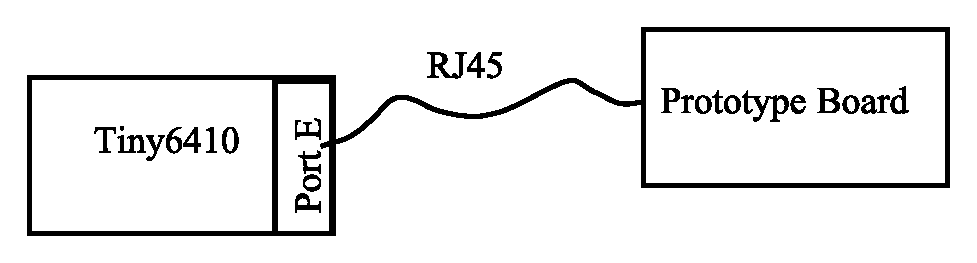
\includegraphics[scale=.50]{BlockDiagram}
	\caption{Block Diagram}\label{BlockDiagram}
\end{figure}


\section{Device Driver}\label{DeviceDriver}
The device driver is the software that operates at the level of the Linux kernel and has direct access to the hardware. The device driver is broken up into three sections,
\begin{enumerate}
	\item Initialization. The control register is set to the correct values as first referenced in section \ref{ARM11HW}. Pseudocode for the initialization can be found in listing \ref{SetGPECONCode}. The driver is also registered with the Linux kernel and can now be found by user level programs.
	\item Clean up. Deregister the driver from the Linux kernel.
	\item I/O Control. The driver needs to provide a method for user level programs to interact with the hardware. The device driver therefore implements the \emph{ioctl} function. The user level control function will send commands to the driver's \emph{ioctl} function to perform some action and the function will return a status or data value. The function has to interact with the GPEDAT register first mentioned in section \ref{ARM11HW} to read and write to the Port E pins.  The pseudocode in listing \ref{ReadGPEDATCode} show how to read and write to GPEDAT.
\end{enumerate}

\begin{lstlisting}[language=C, frame=single, caption=Pseudo Code to Prepare GPECON,label=SetGPECONCode]
	//reset the control register
	writel(0x00, S3C64XX_GPECON) ;
	const GPE1_OFF = 0x00 ;
	const GPE3_ON = 0x1000 ;
	new_value =  GPE1_OFF | GPE3_ON ;
	// now write the new values to the control register
	writel(new_value, S3C64XX_GPECON) ;
\end{lstlisting}

\begin{lstlisting}[language=C, frame=single, caption=Pseudo Code to read and write GPEDAT,label=ReadGPEDATCode]
	// read the current value
	current_value = readl(S3C64XX_GPEDAT) ;
	// Turn off the LED
	new_value = current_value & ~(0x8) ;
	writel(new_value, S3C64XX_GPEDAT) ;
	// Turn on the LED
	new_value = current_value | (0x8) ;
	writel(new_value, S3C64XX_GPEDAT) ;
	// Read the value of the switch
	return (current_value & 0x2) ;
\end{lstlisting}

\section{User Level Program}
The user level program is the software that operates at the level that the user has access to.  Direct access to the hardware is not allowed. As mentioned in the device driver section \ref{DeviceDriver}, the user level program uses \emph{ioctl} to interact with the device driver. The code is straightforward,
\begin{enumerate}
	\item The user invokes their request via a command line argument.  \emph{-r} to read the switch value. \emph{-l} followed by a zero or one to turn on or off the LED.
	\item The program translates the user into a command \emph{ioctl} from the device driver can understand. A common header file is shared between the user level program and the device driver to ensure the commands are consistent between the two programs.
	\item Call \emph{ioctl} with the appropriate command and read the results or error status.
\end{enumerate}
The pseudocode can be found in listing \ref{UserLevelProg}.

\begin{lstlisting}[language=C, frame=single, caption=User Level Pseudo Code,label=UserLevelProg]
	// read the user input and set the command
	if (input == '-r')
		cmd = READ_SWITCH
	else if (input == '-l0' )
		cmd = LED_OFF
	else if (input == '-l1' )
		cmd = LED_ON
	// open the device driver - the user level program is now
	// 'talking' to the device driver
	fd = open("/dev/matthew_leds", 0);
	// call ioctl
	return_value = ioctl(fd, cmd_switch) ;
	// if necessary, process the return value
\end{lstlisting}

\section{Results}
With all of the software written and the hardware assembled it was time to run the software. As mentioned in section \ref{ProtoBoard} the RJ45 connector was not working and therefore jumper wires were used to connect the Tiny6410 to the prototype board. The software and hardware to turn off and on the LED worked as expected. The software and hardware to read the switch did not work. Without a debugger available, the only resource to debug the problem was to use the \emph{printk} function to print messages from the device driver. The following command \textbf{dmesg} was used to see what messages were printed. It was determined that the GPEDAT register always shows 0x16 once the device driver is initialized. The significance of this is that GPE1, GPE2, and GPE4 are always set high. Therefore, the input of switch, as read by the software, will always be on regardless of the physical status of the switch.

\section{Conclusion}
This project encompasses software and hardware and each ware presented it's own challenges. The software challenges were the communication between the user level program and the device driver, as well as understanding the requirements to use the general purpose I/O port E. The hardware challenges proved more formidable with the problems with RJ45 cable as well as the GPE bits set high. Before the next project, the GPE bits will have to be researched and fixed, if possible.


\begin{figure}[h]
	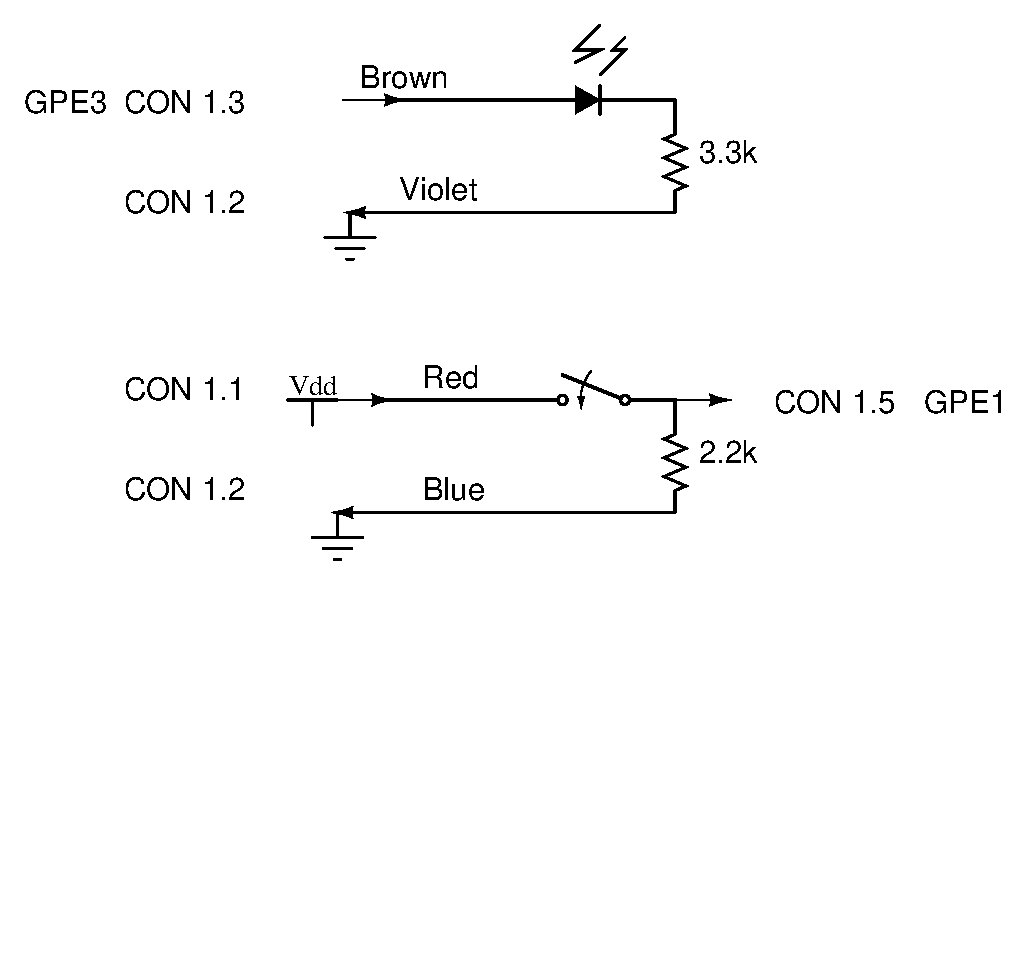
\includegraphics[scale=.55]{lab_1_proto_board}
	\caption{Schemaitic for Prototype Board}\label{lab_1_proto_board}
\end{figure}

\begin{thebibliography}{9}
\bibitem{LDD}
Jonathan Corbet, Alessandro Rubini, and Greg Kroah-Hartman,
\emph{Linux Device Drivers, Third Edition},
O'Reilly Media,
Sebastopol, CA,
2005

\bibitem{Samsung}
-,
\emph{User's Manual \\ S3C6410X \\ RISC Microprocessor},
Samsung Electronics, Inc.,
2008

\bibitem{HWHandout}
Harry Li,
\emph{Handout On Hardware of the ARM11 Development Board},
Computer Engineering Department, College of Engineering,
 San Jose State University,
Spring, 2012
\end{thebibliography}

\end{document}
